\documentclass[12pt]{article}
\usepackage{amssymb}
\usepackage{amsthm}
\usepackage{amsmath}
\usepackage{float}
\usepackage{graphicx}
\usepackage{breqn}
\usepackage[margin=1in]{geometry}
\newcommand{\parder}[2]{\frac{\partial}{\partial{#2}}#1}
\newcommand{\parderpow}[3]{\frac{\partial^{#3}}{\partial{#2}^{#3}}#1}
\newcommand{\parderplace}[2]{\frac{\partial{#1}}{\partial{#2}}}
\newcommand{\parderpowplace}[3]{\frac{\partial^{#3}{#1}}{\partial{#2}^{#3}}}
\newcommand{\Exp}{\mathrm{Exp}}
\newcommand{\bra}[1]{\langle #1}
\newcommand{\ket}[1]{\lvert #1 \rangle}
\newcommand{\highlight}[2]{\colorbox{#2}{$\displaystyle #1$}}
\renewcommand{\thesubsection}{(\alph{subsection})}

\usepackage{minted}
\usepackage[caption=false]{subfig}

\begin{document}
\title{Ph 121a Assignment 3}
\author{Nicholas Meyer}

\maketitle

\section{Vibrating String}

\subsection{Modifications to ODE integrator suite}

It was necessary to modify the integration routines written for assignment
1 to allow for arbitrary boundary conditions. This was achieved by adding
an argument \mintinline{python}/equation_deriv/ that allows the user to choose
whether the equations specify the first derivative of certain variables or
the value of the variables themselves.

Note that it is possible to specify conflicting boundary conditions (i.e.
set the value of $q_j$ to be a sinusoid and set the first time derivative to be
zero); in this case, the behavior is unspecified.

\subsection{Plucked string, fixed ends, no damping}

Without any additional terms, the string conserves energy and exhibits
periodic behavior.

\begin{figure}[H]
  \subfloat{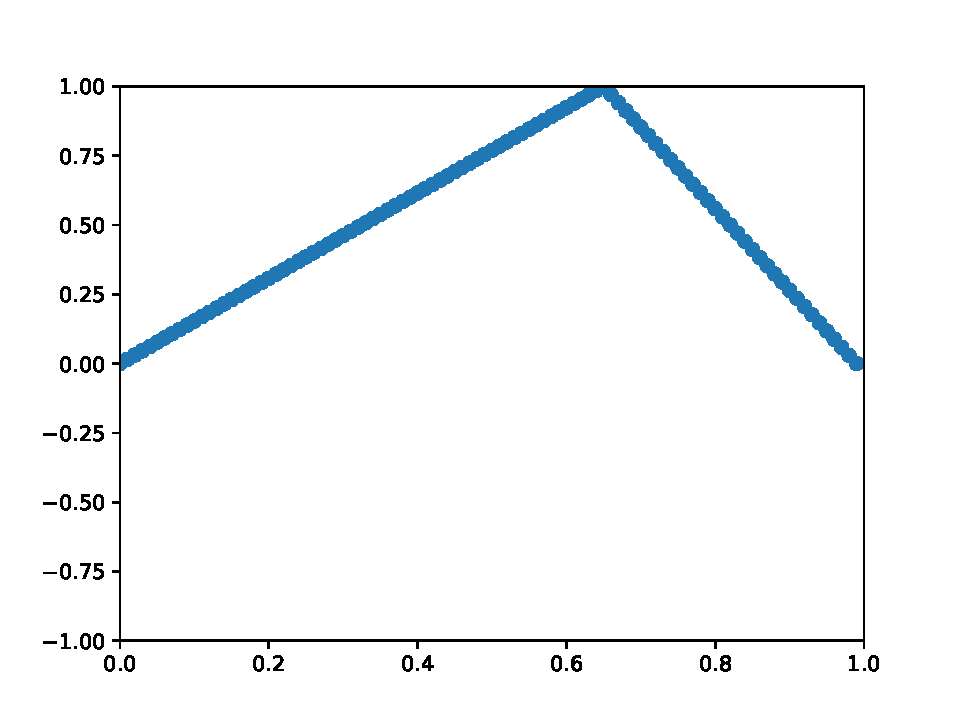
\includegraphics[width=0.5\linewidth]{writeup_plots/plucked_start.pdf}}
  \subfloat{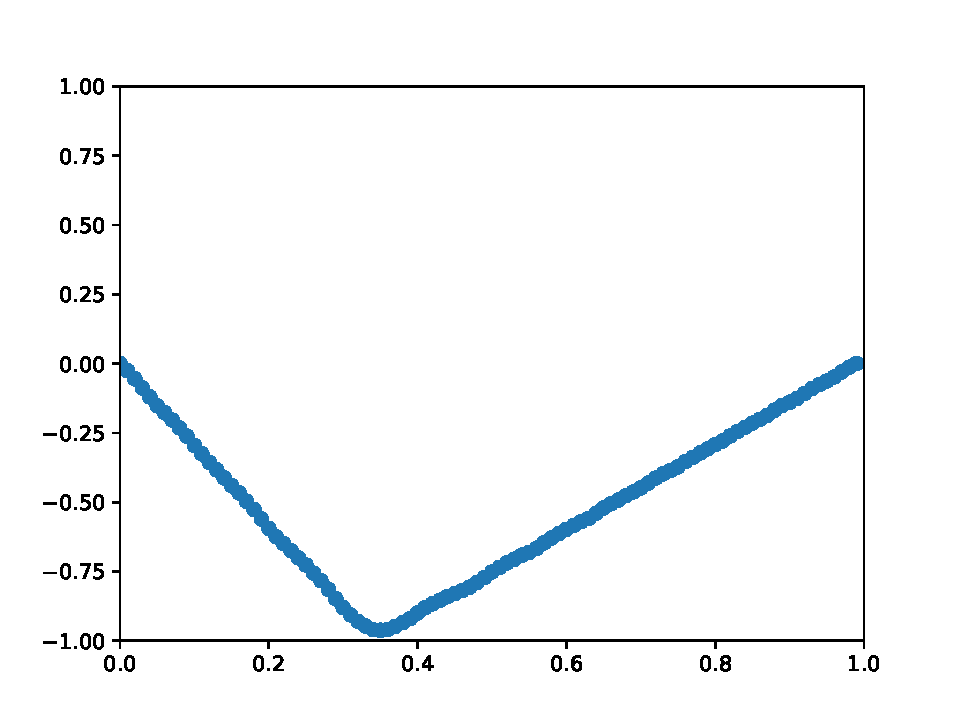
\includegraphics[width=0.5\linewidth]{writeup_plots/plucked_later.pdf}}
  \caption{Left: initial state of the string. Right: state of the string after
    half a period.}
\end{figure}

\subsection{Sinusoidally driven string}

The left end of the string was driven with a sinusoid
$0.25cos{(10t)}$, no damping.

\begin{figure}[H]
  \subfloat{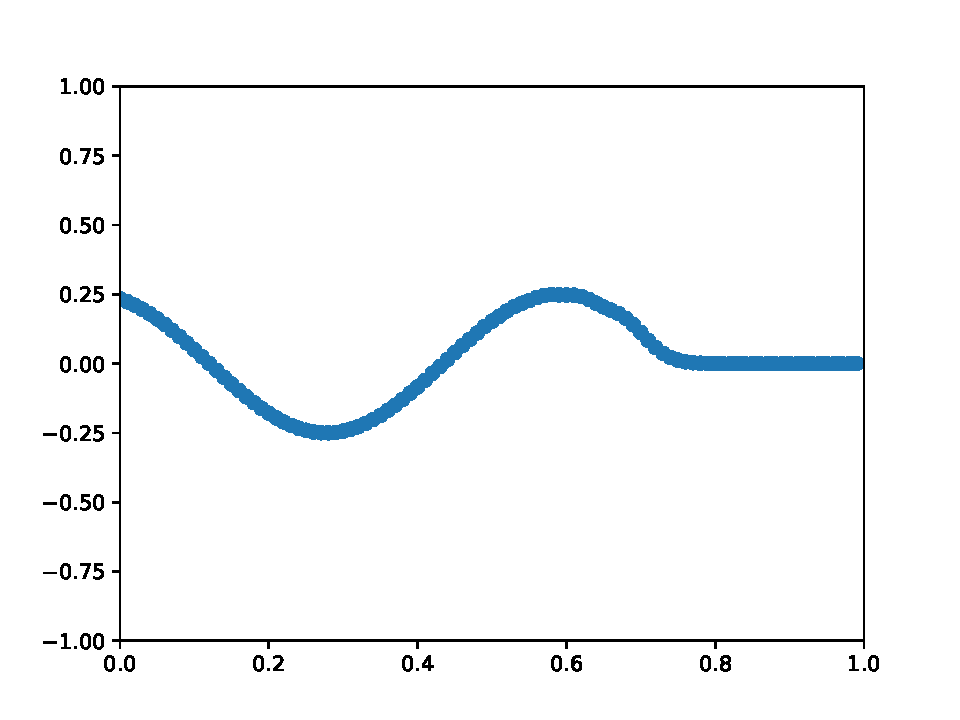
\includegraphics[width=0.5\linewidth]{writeup_plots/sinusoid_start.pdf}}
  \subfloat{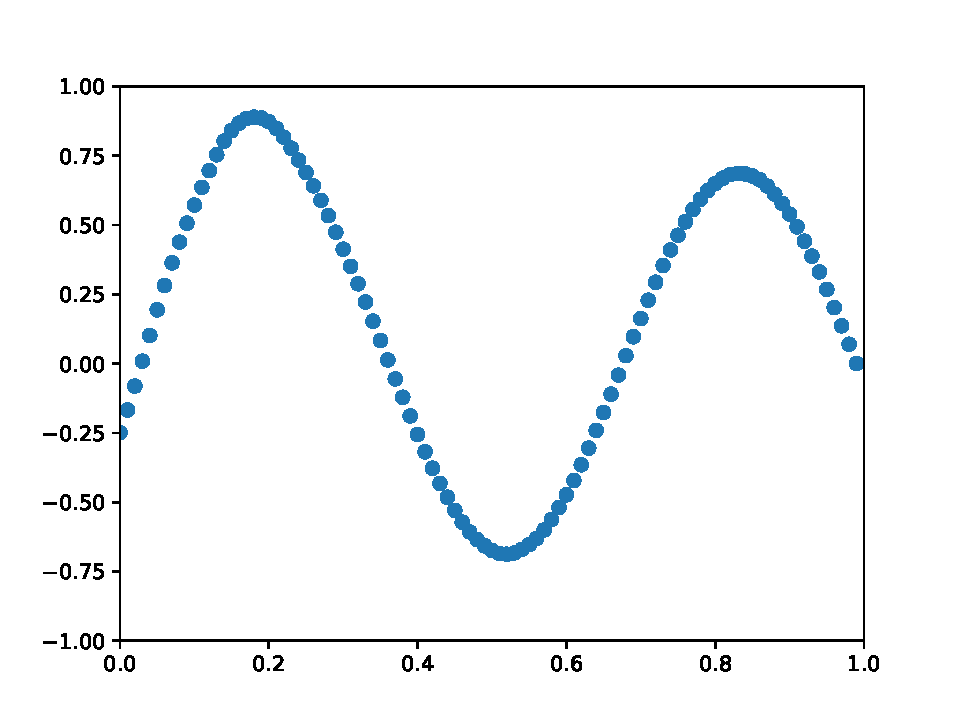
\includegraphics[width=0.5\linewidth]{writeup_plots/sinusoid_later.pdf}}
  \caption{Left: state of the string as the wave propagates to the right.
  Right: development of resonance phenomenon at later time step.}
\end{figure}

\subsection{Damped string}

A damping term of $-\gamma \dot{x} / \rho$ (with $\gamma = 1$) was added
to the regular plucked string to observe a decay in the oscillation amplitude
over time.

\begin{figure}[H]
  \subfloat{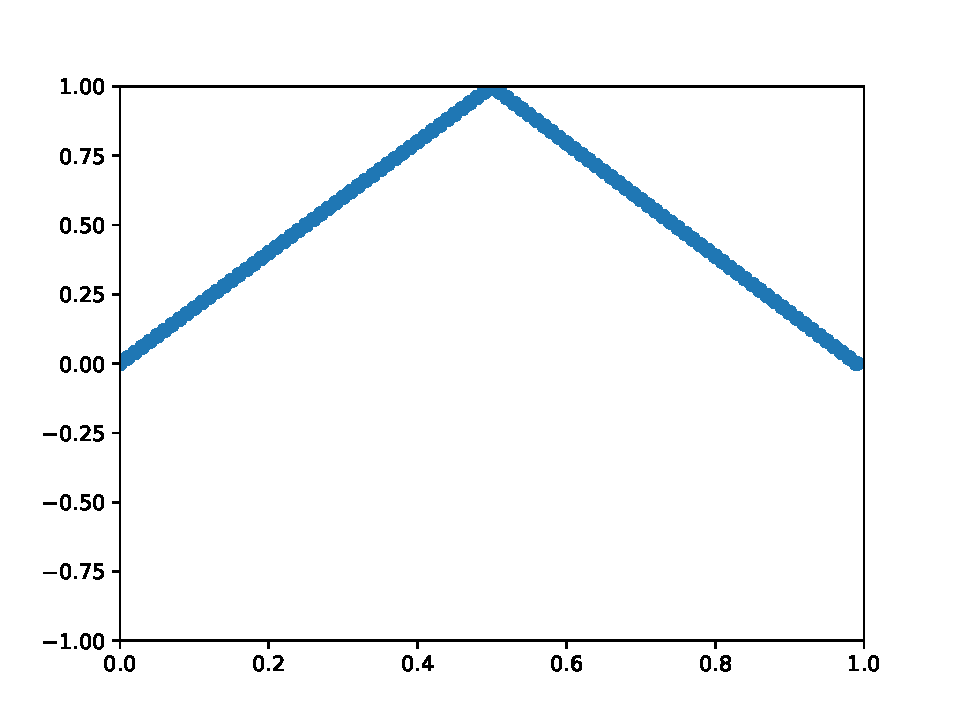
\includegraphics[width=0.5\linewidth]{writeup_plots/damped_start.pdf}}
  \subfloat{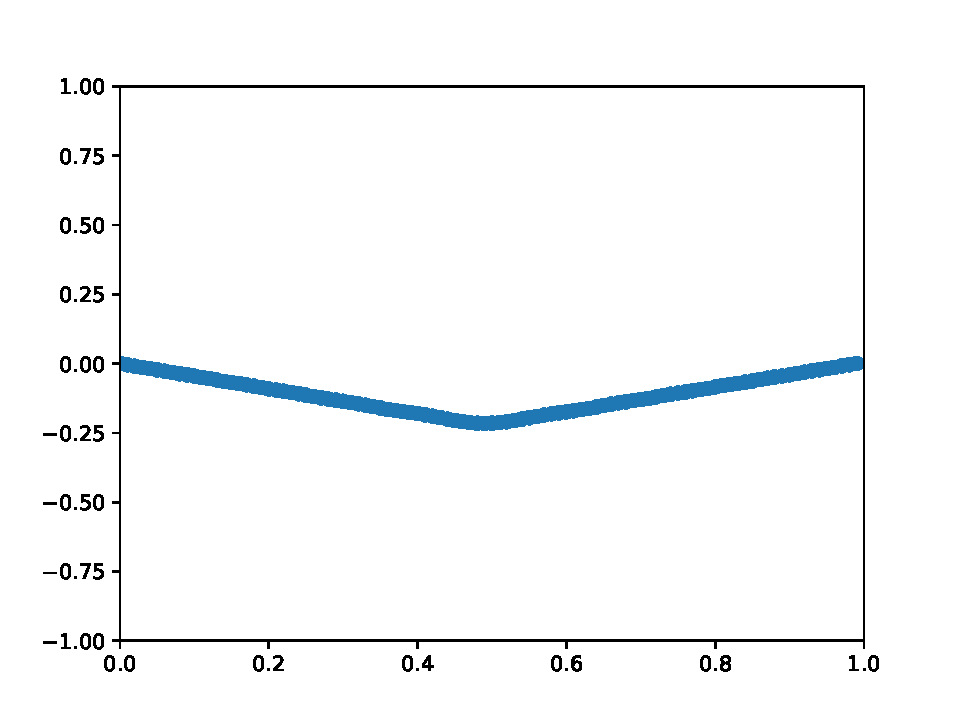
\includegraphics[width=0.5\linewidth]{writeup_plots/damped_later.pdf}}
  \caption{Left: starting pluck for the damped string. Right: lower amplitude peak at later time, evidence of damping.}
\end{figure}

\subsection{Ergodic string}

A nonlinear term $-\lambda \phi^3 / \rho$ was added to the equation of motion of the string, resulting in thermalization.

\begin{figure}[H]
  \subfloat{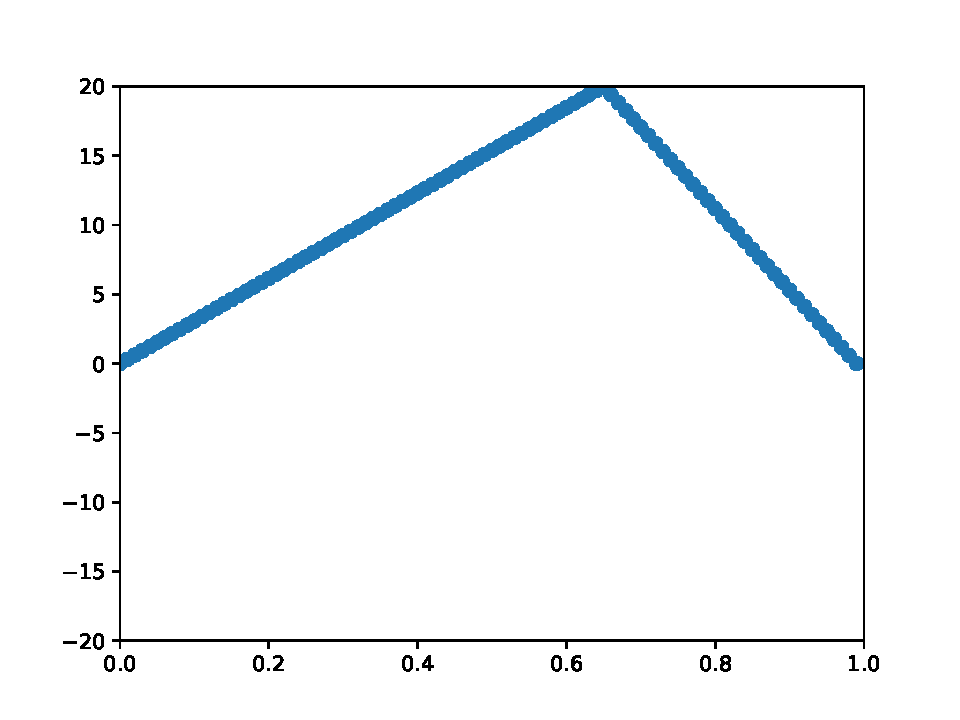
\includegraphics[width=0.5\linewidth]{writeup_plots/ergo_start.pdf}}
  \subfloat{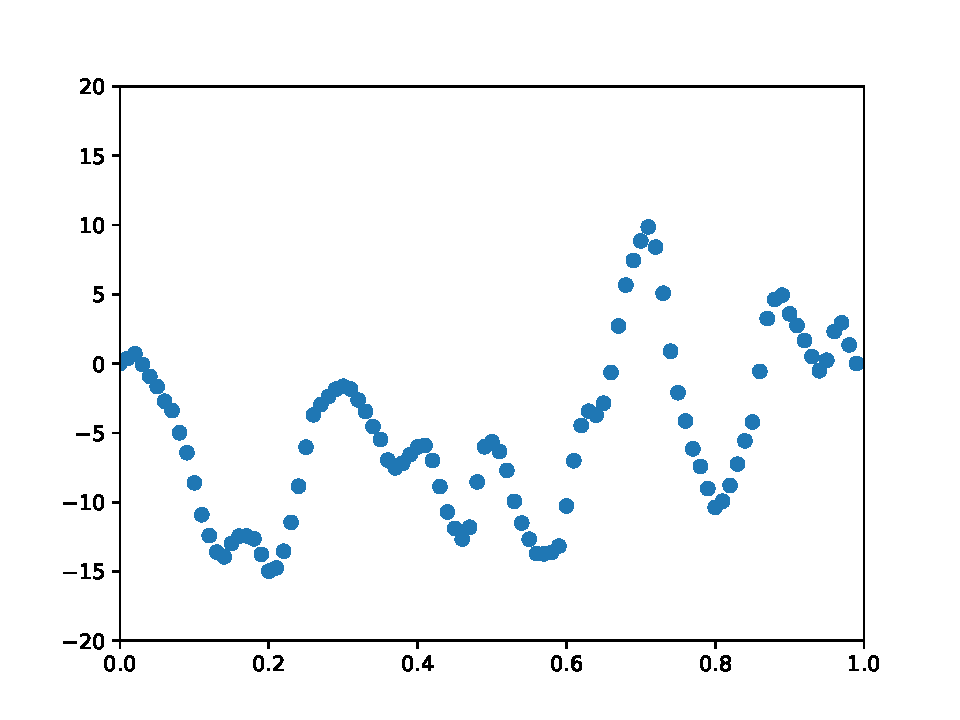
\includegraphics[width=0.5\linewidth]{writeup_plots/ergo_later.pdf}}
  \caption{Left: starting pluck. Right: final state, thermalized.}
\end{figure}

\subsection{Non-ergodic string}

A simulation of a string following the Fermi-Pasta-Ulam-Tsingou equation of
motion was implemented. The expression in terms of finite differences is

\begin{align}
  \ddot{x}_i = \frac{k}{m \delta^2}\left(x_{i - 1} - 2x_i + x_{i + 1}\right)
  \left[1 + \alpha\left(-x_{i - 1} + x_{i + 1}\right)\right]
\end{align}

The alpha parameter was set to $-0.01$. The behavior is periodic up to the
appearance of small oscillations (see animated gif).
Although small oscillations can be seen
to appear as the simulation progresses due to the accumulation of numerical
noise, the behavior is clearly distinct from thermalization.

\begin{figure}[H]
  \subfloat{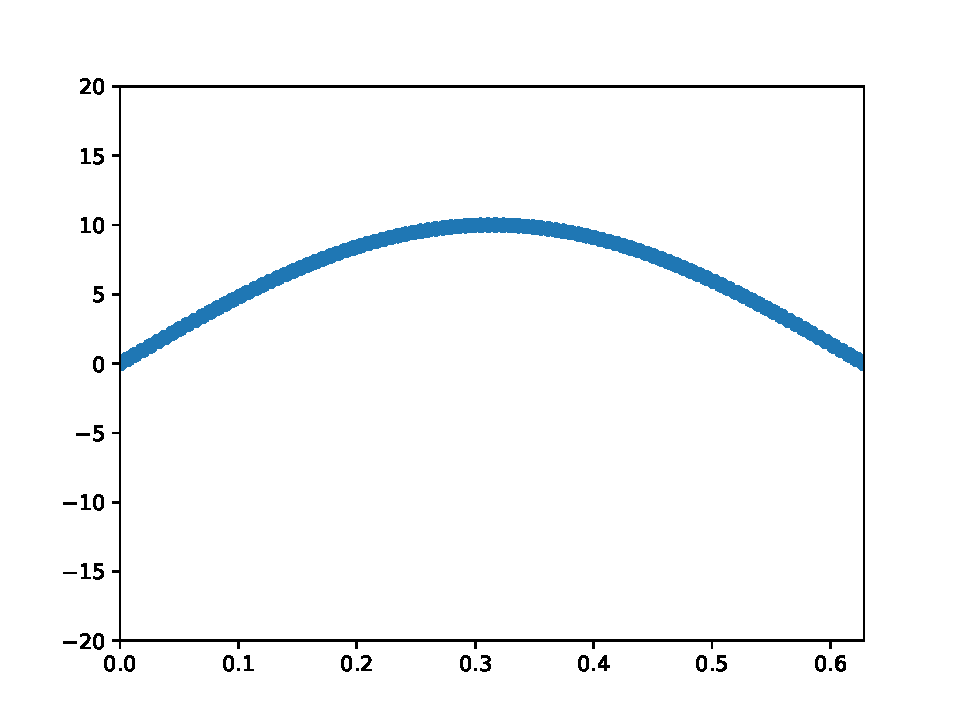
\includegraphics[width=0.8\linewidth]{writeup_plots/nonergo_start.pdf}} \\
  \subfloat{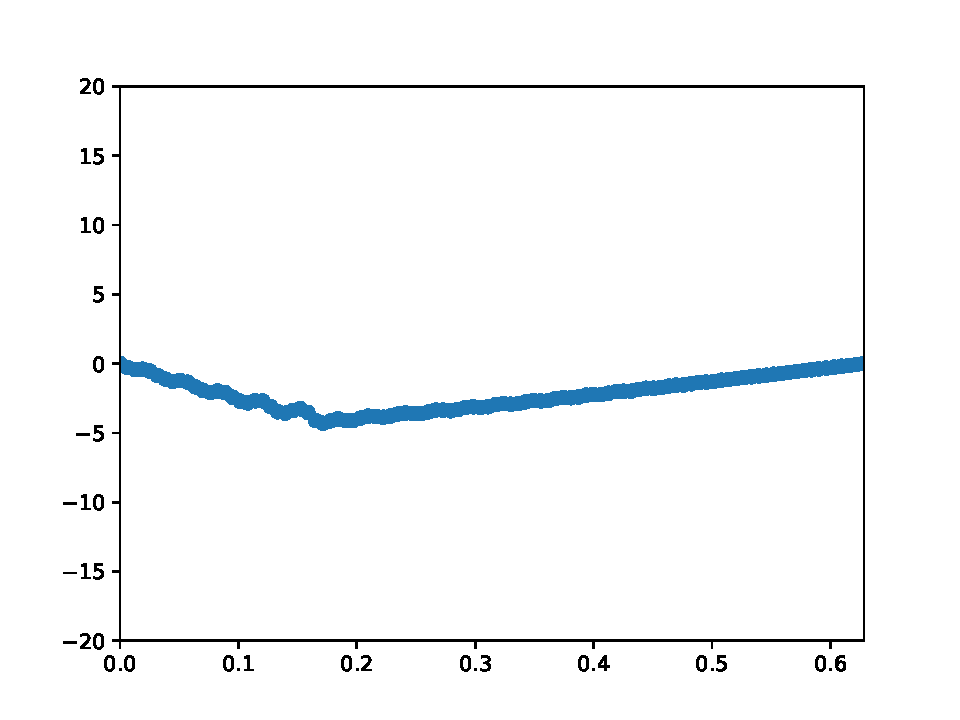
\includegraphics[width=0.4\linewidth]{writeup_plots/nonergo_mid.pdf}}
  \subfloat{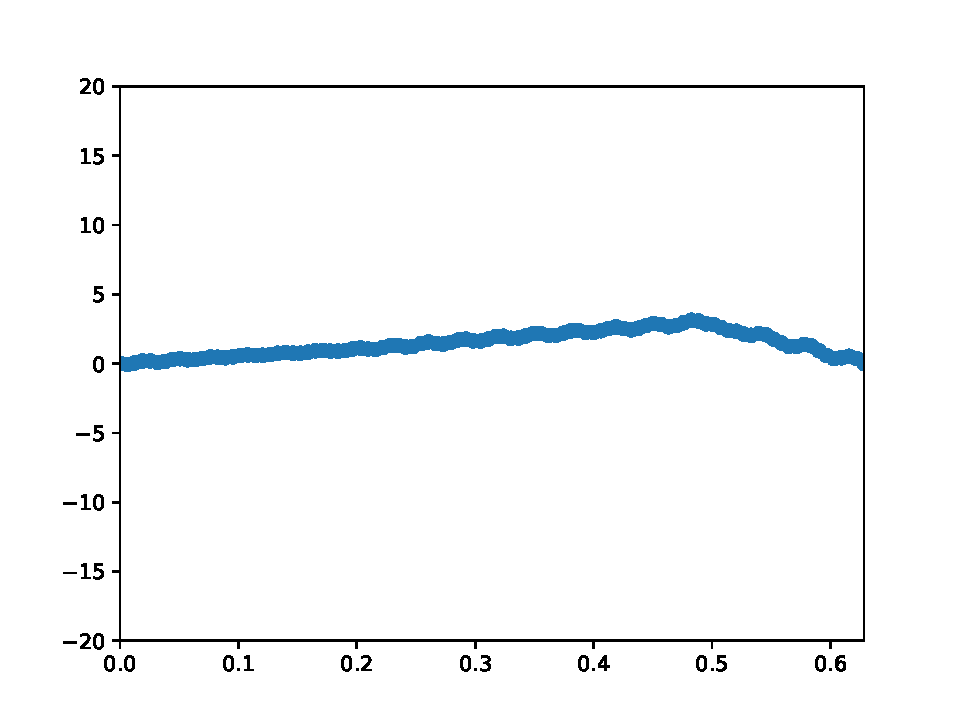
\includegraphics[width=0.4\linewidth]{writeup_plots/nonergo_later.pdf}}
  \caption{Top: Starting configuration. Bottom two plots: the ``crest'' of the
    string travels in a periodic, clockwise, elliptic trajectory.}
\end{figure}

\subsection{Anderson Localization}

To observe anderson localization, the nonlinear term $-\mu \phi / \rho$ was
added to the equation of motion, where $\mu$ assumes uniformly distributed
random values at every point that are fixed in time.

\begin{figure}[H]
  \subfloat{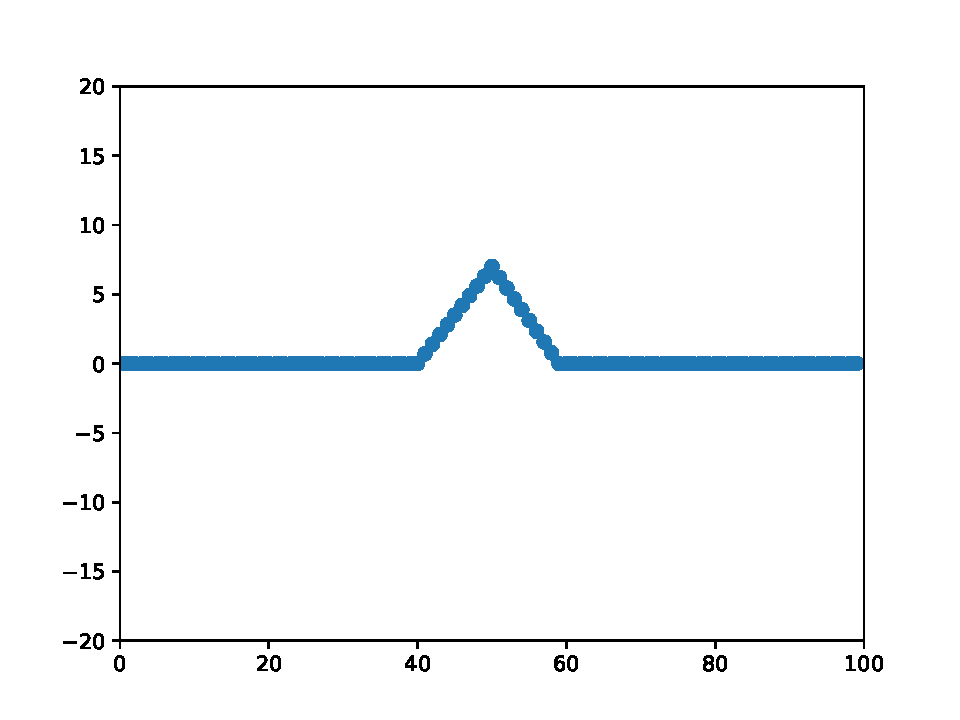
\includegraphics[width=0.5\textwidth]{writeup_plots/anderson_start.pdf}}
  \subfloat{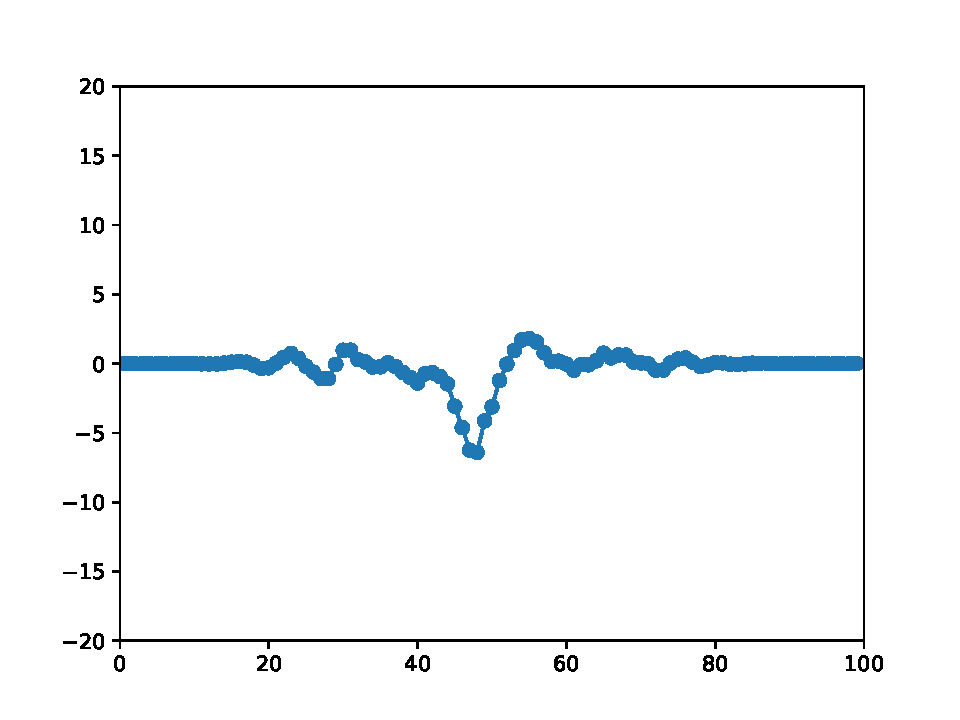
\includegraphics[width=0.5\textwidth]{writeup_plots/anderson_later.pdf}}
  \caption{Left: initial conditions. Right: state of string after several
    oscillations. Wave propagation to the left and right portions of the string
    has been suppressed.}
\end{figure}

\section*{Appendix}

\subsection*{Source Code}

\inputminted{python}{integrator.py}

\newpage

\inputminted{python}{problem.py}

\newpage

\inputminted{python}{physicalstring.py}

\newpage

\inputminted{python}{stringtest.py}

\newpage

\inputminted{python}{testsuite.py}

\end{document}
